\documentclass[conference]{IEEEtran}
\IEEEoverridecommandlockouts
\usepackage{cite}
\usepackage{amsmath,amssymb}
\usepackage{graphicx}
\usepackage{booktabs}
\usepackage{tikz}
\usetikzlibrary{arrows.meta,calc,positioning,fit}
\usepackage{xspace}
\usepackage{url}
\usepackage[hidelinks]{hyperref}

\newcommand{\minADE}{minADE\xspace}
\newcommand{\minFDE}{minFDE\xspace}

\begin{document}

% Truncate long author lists (see references.bib).
\bstctlcite{IEEEexample:BSTcontrol}

\title{LiDAR-Recovered Body Pose Does Not Improve\\
Pedestrian Trajectory Forecasting on Waymo:\\
A Controlled Null and a Detection Floor}

\author{\IEEEauthorblockN{Erik Sch\"utz}
\IEEEauthorblockA{\textit{(affiliation)}\\
\textit{(institution)}\\
(city, country) \\
erik.schuetz@gmx.de}}

\maketitle

\begin{abstract}
Body pose is an intuitively attractive input for pedestrian trajectory
forecasting: gait, stance and facing appear to encode intent that a position
history does not. We test this on the Waymo Open Motion Dataset with SMPL poses
recovered from LiDAR, and find no measurable benefit. The decisive comparison is
not pose against no pose---which confounds body information with the capacity of
an extra input branch---but correct pose against the same architecture fed
\emph{another pedestrian's} pose. On that control the effect is
$+0.66\%$ ($p{=}0.52$) from scratch, $+0.88\%$ ($p{=}0.18$) after full-dataset
pretraining, $-1.02\%$ ($p{=}0.56$) at an intermediate scale and $+0.04\%$
($p{=}0.93$) at $43\times$ more training scenes, while the baseline improves
$19\%$ from data alone; at the largest scale the data bound the content effect to
$\pm1.7\%$. A directed search over the integration code accepted one of $22$
candidates under a truncated proxy, and the pre-registered eight-seed
confirmation that followed returned $-0.04\%$ ($p{=}0.92$). An oracle control rules
out a dead pathway: the same branch, fed the agent's own future instead of its
body, improves \minADE by $34.8\%$.
We then measure why pose does not. Corrupting that oracle with a controlled
angular error gives the pathway a \emph{detection floor}: the gain survives a
median bearing error of $5.5^\circ$ ($p{=}0.0004$) but is already
indistinguishable from zero at $10.2^\circ$, where the ladder's minimum
detectable effect is $6$\,pp. SMPL body facing is accurate to $44.2^\circ$ on the
cue it is supposed to carry, and across seeds the fitted decay predicts at most
$0.3\%$ there against a branch-capacity cost of ${\sim}1.6\%$---so the null is
not a near miss, and the floor is measurable before a modality is integrated.
Corroborating this, the tracker's box heading estimates the same quantity more
accurately ($25.2^\circ$) and pose does not beat it in any range, occlusion or
heading-jitter stratum. Finally, aggregate MPJPE is the wrong acceptance metric
for pose in a perception stack: scored per joint against a mean-pose baseline,
the head's MPJPE looks \emph{better} than either wrist while it carries a tenth
of their skill.
\end{abstract}

\begin{IEEEkeywords}
pedestrian trajectory prediction, human pose estimation, LiDAR, autonomous
driving, negative results
\end{IEEEkeywords}

\section{Introduction}
Predicting where a pedestrian will go is a safety-critical function of an
automated vehicle, and body pose is an obvious candidate input. A person's stance,
gait phase and facing direction plausibly reveal intent before their position
changes, and modern perception stacks already produce human mesh or keypoint
estimates. Several recent systems condition trajectory forecasts on pose.

This paper reports that, on the Waymo Open Motion Dataset (WOMD), pose
conditioning does not measurably improve pedestrian trajectory accuracy---and,
more usefully for practitioners, identifies a specific reason that can be
checked quantitatively, and cheaply, before a modality is integrated at all.

We make three contributions.

\textbf{A controlled null.} We measure pose conditioning against a shuffled-pose
control: the same architecture receiving a different pedestrian's body motion.
This isolates information content from the capacity cost of an extra branch, and
it is the comparison a practitioner should demand before adopting any auxiliary
modality. The control is null at three training scales; across six pose
encodings ($6$D joint rotations, 3D joint positions, root-orientation-free,
agent-frame root, constant-pose and eight frame-invariant descriptors) and two
encoder architectures (GRU and cross-attention); under two integration styles,
a directed architecture search, and a pre-registered eight-seed confirmation on a
held-out split. An oracle arm, which
replaces the body with a signal encoding the agent's own future, improves
\minADE by $34.8\%$ through the same branch---so the null is a property of pose,
not of the plumbing.

\textbf{A detection floor.} We then measure how accurate a side channel must be
before this pathway converts it into accuracy at all, by corrupting that oracle
with a controlled angular error. The gain decays by roughly half for every
$3$--$8^\circ$ of bearing error: it is still significant at $5.5^\circ$ and is
already indistinguishable from zero at $10.2^\circ$. SMPL body facing is accurate
to $44.2^\circ$ on the cue it is supposed to carry, where every seed's fitted
decay predicts a gain under $0.3\%$ against a branch cost of ${\sim}1.6\%$. The
null is not a near miss, and the floor can be measured before any modality is
integrated.

\textbf{A measurement caveat.} Aggregate MPJPE cannot distinguish a pose
estimator that tracks a joint imprecisely from one that ignores the input and
emits its prior. Scoring each joint against an always-predict-the-mean-pose
baseline, MPJPE is uninformative about which joints are actually recovered
($\rho{=}-0.11$ across joints, n.s.) and inverts the ordering for the head.
Accepting a pose estimator into an AV stack on a single error number risks
importing a prior.

We also report, as a cautionary note, that our first attempt at this study was
invalidated by an export bug that silently substituted other pedestrians'
bodies---a failure any pose pipeline keyed by object identity can reproduce.

\section{Related Work}
Trajectory forecasting on WOMD is dominated by anchor- and query-based
transformers; we build on MTR~\cite{shi2022mtr,shi2023mtrpp}, which is
representative and strong. Human mesh recovery from LiDAR is
maturing~\cite{fan2023lidarhmr}, with motion priors used to complete sparse
observations~\cite{rempe2021humor,he2022nemf,mahmood2019amass}. Intent-focused
work on pedestrian datasets~\cite{rasouli2019pie,fang2018pedestrian} targets
crossing decisions rather than metric trajectories.

\textbf{Relation to prior positive results.} Pose conditioning has reported real
gains, and our mechanism predicts where they come from rather than contradicting
them. Social-Transmotion~\cite{saadatnejad2024socialtransmotion} lowers ADE on
the synthetic JTA dataset from $0.99$ to $0.89$ with \emph{ground-truth} 3D pose,
and---the harder case for us---from $0.40$ to $0.36$ on JRDB with
\emph{estimated} pose. Social-Pose~\cite{gao2025socialpose} reports about $25\%$
on JTA ($1.20{\to}0.90$) and on JRDB. Salzmann et al.~\cite{salzmann2023robots}
report ${\approx}10\%$ from onboard-estimated keypoints at ranges up to $7$\,m,
specifically for agents with little position history, which is also our best
hypothesis.

The most informative comparison is within Social-Pose itself. Alongside JTA it
evaluates on Pedestrians and Cyclists in Road Traffic, the one vehicle-captured
dataset in that study, and there---with \emph{ground-truth} 3D pose---ADE moves
from $0.58$ to $0.57$\,m, and by $0.01$\,m or less for every one of the five
architectures tested, against the ${\approx}25\%$ the same encoder delivers on
JTA. The authors attribute this to the shorter horizon and the absence of
interacting neighbours; our measurements suggest an additional reason that
travels with the sensor rather than the horizon. Either way, the closest
published setting to ours already reports approximately our result.

Two properties separate the remaining positive settings from an AV stack, and
both follow from the mechanism in Sec.~\ref{sec:why}. \emph{Range and sensor:}
JRDB is an indoor and campus robot dataset in which pedestrians are metres away
and pose is camera-derived, whereas WOMD pedestrians are observed from $2$ to
$75$\,m and often return a few dozen LiDAR points. \emph{The baseline:} those
predictors consume positions, not a tracker's box heading, so body facing is new
information there and partly duplicated here. On controls, none reports a
shuffled-pose arm---though the confound differs by design. Social-Transmotion
trains one network with modality masking and reads both input sets off the same
weights, so no extra parameters are involved there; architectures that add a
dedicated pose branch do pay the capacity cost we measure ($+1.7\%$ \minADE),
which is the same order as the smaller reported gains. Our contribution is not
an architecture but a controlled measurement of whether the modality pays in an
AV setting, with the reason it does not.


\begin{figure*}[t]
\centering
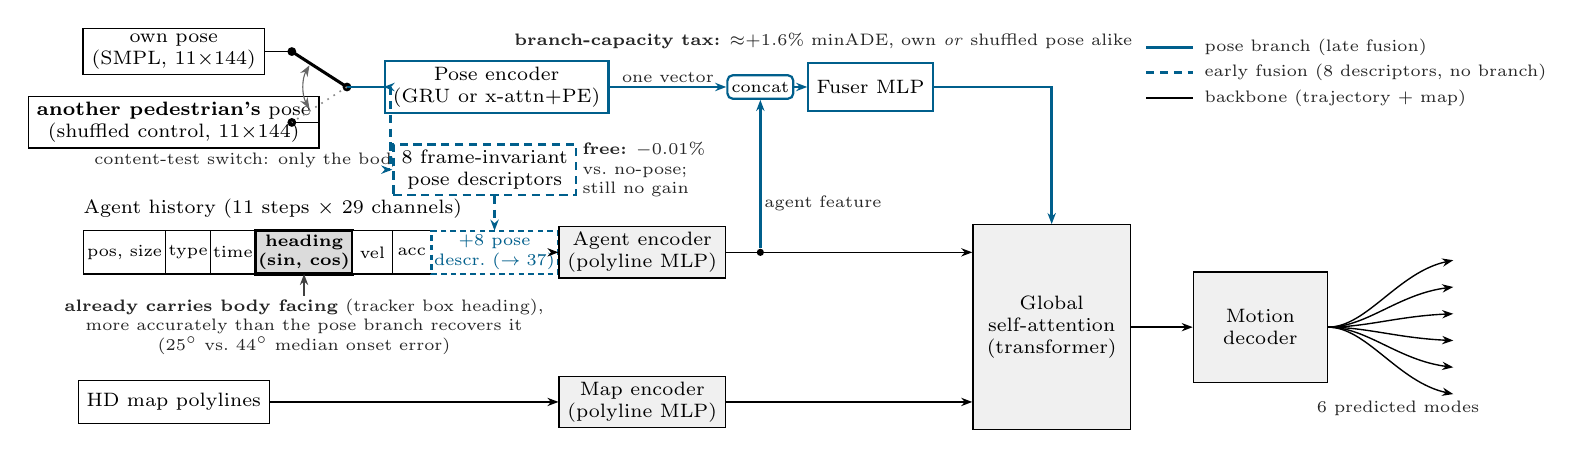
\begin{tikzpicture}[
  x=1cm, y=1cm,
  font=\scriptsize,
  >={Stealth[length=4pt,width=3pt]},
  % --- styles -------------------------------------------------------------
  blk/.style={draw=black, line width=0.5pt, fill=black!6, align=center,
              inner xsep=3pt, inner ysep=2pt, minimum height=0.6cm},
  pblk/.style={blk, fill=white, draw=figaccent, line width=0.8pt},
  src/.style={blk, fill=white, minimum width=2.3cm, minimum height=0.55cm},
  annfont/.style={font=\fontsize{6}{7}\selectfont},
  cell/.style={draw=black, line width=0.4pt, fill=white, annfont, align=center,
               inner sep=1pt, outer sep=0pt, minimum height=0.55cm},
  bb/.style={draw=black, line width=0.5pt, ->},
  late/.style={draw=figaccent, line width=1pt, ->},
  early/.style={draw=figaccent, line width=1pt, dash pattern=on 3pt off 2pt, ->},
  ann/.style={annfont, align=center, text=black!85, inner sep=1pt},
  tap/.style={circle, fill=black, inner sep=0pt, minimum size=2.6pt},
]
\definecolor{figaccent}{RGB}{0,95,140}

% =========================================================================
% (1) POSE INPUT: own pose vs. another pedestrian's pose, selected by a switch
% =========================================================================
\node[src] (own) at (1.35,5.55) {own pose\\(SMPL, $11{\times}144$)};
\node[src] (oth) at (1.35,4.65) {\textbf{another pedestrian's} pose\\(shuffled control, $11{\times}144$)};
\coordinate (tA) at (2.85,5.55);
\coordinate (tB) at (2.85,4.65);
\coordinate (piv) at (3.55,5.1);
\coordinate (split) at (4.1,5.1);
\draw[line width=0.5pt] (own.east) -- (tA);
\draw[line width=0.5pt] (oth.east) -- (tB);
\fill (tA) circle (1.6pt);
\fill (tB) circle (1.6pt);
\fill (piv) circle (1.6pt);
\draw[line width=1.1pt] (piv) -- (tA);                       % lever: own pose selected
\draw[line width=0.6pt, black!45, dotted] (piv) -- (tB);      % alternative lever position
\draw[<->, black!60, line width=0.4pt]
  (piv) ++(150:0.55) arc[start angle=150, end angle=210, radius=0.55];
\node[ann, anchor=west] at (0.3,4.17) {content-test switch: only the body differs};
\draw[figaccent, line width=1pt] (piv) -- (split);

% =========================================================================
% (3a) LATE FUSION: pose branch -> concat with agent feature -> fuser MLP
% =========================================================================
\node[pblk, minimum width=1.9cm] (penc) at (5.45,5.1) {Pose encoder\\(GRU or x-attn$+$PE)};
\node[pblk, rounded corners=2pt, annfont, inner sep=1.5pt, minimum height=0.3cm] (cat) at (8.8,5.1) {concat};
\node[pblk, minimum width=1.4cm] (fuse) at (10.2,5.1) {Fuser MLP};
\draw[late] (split) -- (penc.west);
\draw[late] (penc) -- node[above, ann] {one vector} (cat);
\draw[late] (cat) -- (fuse);
\node[ann, anchor=south] at (9.6,5.55)
  {\textbf{branch-capacity tax:} ${\approx}{+}1.6\%$ minADE, own \emph{or} shuffled pose alike};

% =========================================================================
% (3b) EARLY FUSION: 8 frame-invariant descriptors appended to agent channels
% =========================================================================
\node[pblk, minimum width=2.1cm, minimum height=0.5cm, dash pattern=on 3pt off 2pt] (desc) at (5.3,4.05)
  {8 frame-invariant\\pose descriptors};
\draw[early] (split) |- (desc.west);
\node[ann, anchor=west, align=left] at (6.5,4.05)
  {\textbf{free:} $-0.01\%$\\vs.\ no-pose;\\still no gain};

% =========================================================================
% (2) AGENT HISTORY with heading channel called out
% =========================================================================
\node[font=\scriptsize, anchor=west, inner sep=0pt] at (0.2,3.55)
  {Agent history ($11$ steps $\times$ $29$ channels)};
\node[cell, minimum width=1.05cm, anchor=west] (c1) at (0.2,3.0) {pos, size};
\node[cell, minimum width=0.55cm, anchor=west] (c2) at (c1.east) {type};
\node[cell, minimum width=0.55cm, anchor=west] (c3) at (c2.east) {time};
\node[cell, minimum width=1.1cm, anchor=west, fill=black!14, line width=1.3pt,
      font=\fontsize{6}{7}\selectfont\bfseries] (c4) at (c3.east)
  {heading\\(sin, cos)};
\node[cell, minimum width=0.5cm, anchor=west] (c5) at (c4.east) {vel};
\node[cell, minimum width=0.5cm, anchor=west] (c6) at (c5.east) {acc};
\node[cell, minimum width=1.3cm, anchor=west, draw=figaccent, text=figaccent,
      line width=0.8pt, dash pattern=on 2pt off 1.5pt] (c7) at (c6.east)
  {$+8$ pose\\descr.\ ($\to 37$)};
\draw[early] (desc.south -| c7) -- (c7.north);

\node[ann, anchor=north] (hann) at (c4.south |- 0,2.45)
  {\textbf{already carries body facing} (tracker box heading),\\
   more accurately than the pose branch recovers it\\
   ($25^\circ$ vs.\ $44^\circ$ median onset error)};
\draw[black!75, line width=0.5pt, ->] (hann.north) -- (c4.south);

% =========================================================================
% (4) BACKBONE: encoders -> global self-attention -> motion decoder -> 6 modes
% =========================================================================
\node[blk, minimum width=1.8cm] (aenc) at (7.3,3.0) {Agent encoder\\(polyline MLP)};
\node[src] (map) at (1.35,1.1) {HD map polylines};
\node[blk, minimum width=1.8cm] (menc) at (7.3,1.1) {Map encoder\\(polyline MLP)};
\node[blk, minimum width=2.0cm, minimum height=2.6cm] (tr) at (12.5,2.05)
  {Global\\self-attention\\(transformer)};
\node[blk, minimum width=1.7cm, minimum height=1.4cm] (dec) at (15.15,2.05) {Motion\\decoder};

\draw[bb] (c7.east) -- (aenc.west);
\draw[bb] (map.east) -- (menc.west);
\draw[bb] (aenc.east) -- (tr.west |- aenc);
\draw[bb] (menc.east) -- (tr.west |- menc);
\draw[bb] (tr.east) -- (dec.west);

% late-fusion detour: tap the agent feature, fuse, re-enter the transformer
\node[tap] (tp) at (8.8,3.0) {};
\draw[late] (tp) -- node[right, ann, pos=0.3] {agent feature} (cat);
\draw[late] (fuse.east) -| (tr.north);

% six predicted modes
\foreach \k in {0,...,5} {
  \draw[bb] (dec.east) .. controls (16.5,2.05) and (16.9,{2.05+(\k-2.5)*0.28}) ..
    (17.6,{2.05+(\k-2.5)*0.34});
}
\node[ann, anchor=north] at (16.9,1.15) {6 predicted modes};

% =========================================================================
% legend
% =========================================================================
\begin{scope}[shift={(13.7,5.6)}]
  \draw[late,-]  (0,0)    -- (0.6,0);    \node[ann, anchor=west] at (0.7,0)    {pose branch (late fusion)};
  \draw[early,-] (0,-0.32) -- (0.6,-0.32); \node[ann, anchor=west] at (0.7,-0.32) {early fusion (8 descriptors, no branch)};
  \draw[bb,-]    (0,-0.64) -- (0.6,-0.64); \node[ann, anchor=west] at (0.7,-0.64) {backbone (trajectory $+$ map)};
\end{scope}
\end{tikzpicture}

\caption{The two arms differ only in \emph{whose} body enters the model. The
content-test switch~(1) feeds the predictor either the pedestrian's own SMPL
sequence or another pedestrian's, holding parameters, optimiser and input
dimensionality fixed; everything downstream is shared. Blue: MTR, unchanged;
orange: added for pose. The agent-history strip shows that the tracker's box
heading is \emph{already} an input. Solid orange~(2): the pose branch (late
fusion), which costs ${\approx}1.6\%$ \minADE whether it carries the right body
or the wrong one; dashed~(3): early fusion, which removes that cost and still
yields no benefit.}
\label{fig:arch}
\end{figure*}

\section{Setup}
\label{sec:setup}

\subsection{Data and a data-integrity failure}
We use WOMD~\cite{ettinger2021waymo} with SMPL~\cite{loper2015smpl} poses
recovered from LiDAR by the Waymo-3DSkelMo pipeline~\cite{zhu2025waymo3dskelmo},
which fits per-frame bodies with LiDAR-HMR~\cite{fan2023lidarhmr} and completes
them using AMASS-trained motion
priors~\cite{mahmood2019amass,rempe2021humor,he2022nemf}. Poses cover the $11$
observed frames; the prediction horizon is $8$\,s at $10$\,Hz. The branch is not
starved: every predicted agent carries at least one valid pose frame, and
$86.7\%$ of observed frames carry one, so sparsity of pose is not an explanation
for anything that follows.

One property of that pipeline bears on Sec.~\ref{sec:why}: when a pedestrian is
moving and the raw LiDAR estimate of root rotation deviates from the
past-trajectory direction by more than $90^\circ$, the pipeline snaps the root to
the direction of travel. Body facing is therefore partly trajectory-derived for
moving pedestrians. This reinforces the redundancy we report rather than
weakening it, and it does not reach the stationary-onset analysis, whose events
are all below $0.3$\,m/s.

Our first pass at this study was invalid. The export keyed pose clips by a
scene-\emph{local} object identifier, so clips collided across scenes and nearly
every training sequence carried another pedestrian's body. A per-scene re-export
($299{,}220$ scenes, $1.81$M sequences) cut the median error between root heading
and travel direction from $41.5^\circ$ to $11.4^\circ$ and raised the
gait--speed correlation from $r{=}0.26$ to $0.58$. We report it because the
failure is silent---training converges, losses look normal---and identity-keyed
joins are common in pose pipelines. Every number here is from the corrected
export.

\subsection{Arms and the content test}
Three arms share one architecture (Fig.~\ref{fig:arch}). \emph{No-pose} receives trajectories and map.
\emph{Pose} adds the pedestrian's own SMPL sequence. \emph{Shuffled} receives
another pedestrian's sequence, with identical parameter count, optimiser and
input dimensionality. A fourth arm, \emph{oracle}, replaces the SMPL features with a six-channel
encoding of the agent's own future displacement at $3$ and $8$\,s, leaving the
branch and its masks untouched; it shows the pathway can carry information at
all (Sec.~\ref{sec:poscontrol}).

Pose versus no-pose confounds information with branch capacity; pose versus
shuffled isolates content. We call the latter the \emph{content test} and treat it
as decisive. Relative differences are $(A-B)/B$; negative favours $A$.

Inference is over \emph{seeds}, which is the unit the treatment is applied to:
every comparison between trained arms is a paired $t$-test on per-seed
differences. The two exceptions are flagged where they occur---per-pedestrian
subpopulation tests and the per-joint intervals of Table~\ref{tab:skill}, which
resample pedestrians. We also report a hierarchical bootstrap that resamples seeds and
then pedestrians, and it agrees; we do not quote a percentile bootstrap
$p$-value, because with five seeds whose differences share a sign it returns the
resolution floor $1/N_{\text{boot}}$ rather than a calibrated tail probability,
and a pedestrian-only bootstrap ignores between-seed variance entirely.

\subsection{Protocol}
\label{sec:protocol}
Every arm trains for $30$ epochs with AdamW (batch $2$ per GPU, weight decay
$0.01$, gradient-norm clipping $1.0$) under a step schedule that halves the
learning rate at epochs $10$, $20$ and $25$; the decoder predicts $K{=}6$ modes.
The learning rate is chosen per rung from a grid run separately for each arm:
$1{\times}10^{-4}$ at $579$ scenes, $5{\times}10^{-5}$ at $5$k and
$2.5{\times}10^{-5}$ at $25$k, where every arm peaks at the same interior
optimum. Validation is fixed at $5{,}171$ scenes and $16{,}486$ pedestrians; the
directed search of Sec.~\ref{sec:search} splits it once into a development half
($2{,}617$ scenes, $8{,}445$ agents) and a held-out half ($2{,}554$ scenes,
$8{,}041$ agents). Headline numbers are taken at each run's best validation epoch
over a fixed evaluation schedule, and Sec.~\ref{sec:real} reports what changes
under a fixed-epoch rule. Official WOMD mAP and gated miss rate need the full
retained prediction set, which our per-epoch evaluation does not store, so we
report \minADE, \minFDE and miss rate at $2$\,m. Code, configs, per-seed metrics
and the analysis scripts are released with the paper.

\section{Results}

\begin{table}[t]
\caption{Content test across training scale, validation fixed. The learning rate
is selected per rung by a grid run separately for every arm; all arms peak at the
same value (Sec.~\ref{sec:protocol}). Percentages are differences of arm means;
$p$-values are paired $t$-tests over per-seed differences. Negative favours pose.}
\label{tab:ladder}
\centering
\footnotesize
\begin{tabular}{lccc}
\toprule
Training scenes & $579$ & $5$k & $25$k \\
Pedestrians & $6{,}348$ & $31{,}302$ & $142{,}807$ \\
Seeds & $5$ & $3$ & $5$ \\
\midrule
\multicolumn{4}{l}{\emph{\minADE} (m)} \\
No-pose  & $0.4599$ & $0.4176$ & $0.3716$ \\
Pose     & $0.4620$ & $0.4138$ & $0.3778$ \\
Shuffled & $0.4589$ & $0.4181$ & $0.3777$ \\
Pose vs.\ no-pose & $+0.45\%$ & $-0.90\%$ & $+1.66\%^{*}$ \\
\textbf{Content test} & $+0.66\%$ & $-1.02\%$ & $+0.04\%$ \\
$p$ (content) & $0.52$ & $0.56$ & $0.93$ \\
\midrule
\multicolumn{4}{l}{\emph{\minFDE} (m)} \\
No-pose  & $0.9922$ & $0.8992$ & $0.8049$ \\
Pose     & $0.9824$ & $0.8875$ & $0.8131$ \\
Shuffled & $0.9780$ & $0.8900$ & $0.8104$ \\
Pose vs.\ no-pose & $-0.99\%$ & $-1.30\%$ & $+1.02\%^{\dagger}$ \\
\textbf{Content test} & $+0.45\%$ & $-0.28\%$ & $+0.33\%$ \\
$p$ (content) & $0.63$ & $0.83$ & $0.61$ \\
\bottomrule
\multicolumn{4}{l}{\footnotesize $^{*}t(4){=}10.3$, $p{=}5{\times}10^{-4}$; the shuffled arm} \\
\multicolumn{4}{l}{\footnotesize pays the same cost, $+1.63\%$, $t(4){=}2.8$, $p{=}0.048$.} \\
\multicolumn{4}{l}{\footnotesize $^{\dagger}t(4){=}6.1$, $p{=}0.004$.}
\end{tabular}
\end{table}


\begin{table}[t]
\caption{Clean core at $579$ scenes, $n{=}5$ seeds, both regimes. The shuffled arm
has the lowest mean in both: another pedestrian's body is nominally the best input.}
\label{tab:core}
\centering
\footnotesize
\begin{tabular}{llcc}
\toprule
Arm & Per-seed \minADE & Mean $\pm$ sd & Content \\
\midrule
\multicolumn{4}{l}{\emph{From scratch}} \\
No-pose  & $.458\ .443\ .453\ .495\ .450$ & $0.4599 \pm 0.0206$ & --- \\
Shuffled & $.454\ .467\ .451\ .455\ .467$ & $0.4589 \pm 0.0075$ & --- \\
Pose     & $.471\ .456\ .453\ .457\ .474$ & $0.4620 \pm 0.0094$ & $+0.66\%$ \\
\midrule
\multicolumn{4}{l}{\emph{Fine-tuned on a full-WOMD backbone}} \\
No-pose  & $.372\ .366\ .367\ .373\ .368$ & $0.3692 \pm 0.0031$ & --- \\
Shuffled & $.364\ .363\ .364\ .374\ .373$ & $0.3676 \pm 0.0055$ & --- \\
Pose     & $.364\ .372\ .371\ .374\ .373$ & $0.3708 \pm 0.0040$ & $+0.88\%$ \\
\bottomrule
\end{tabular}
\end{table}

\subsection{The null, and its bound}
Table~\ref{tab:ladder} trains all three arms at three scales. Data alone improves
the baseline by $19.2\%$; the content test is null at every rung, in \minADE and
in \minFDE alike, and in miss rate at $2$\,m, where the content test is
$+2.3\%$ at $25$k ($p{=}0.21$) and $+4.5\%$ fine-tuned ($p{=}0.19$)---null, and
with its sign against pose on all three metrics. The rungs are not equally
sensitive, and we state what each one
could have seen: at $80\%$ power the minimum detectable content effect is
$3.5\%$ at $579$ scenes ($n{=}5$), $7.6\%$ at $5$k ($n{=}3$) and $2.2\%$ at
$25$k ($n{=}5$). The $5$k rung is therefore weak evidence on its own and we do
not count it as an independent null; the weight falls on $25$k and on the
eight-seed confirmation of Sec.~\ref{sec:search}. At $25$k the paired seed-level
interval on the content difference is $[-1.59\%,+1.70\%]$, so at the largest
scale we train the data exclude a content effect beyond roughly $1.7\%$ in either
direction---a bound tighter than the $1.6\%$ cost of the branch that would carry
it. The
pedestrian-resampling bootstrap gives a visibly narrower interval
($[-0.0040,+0.0047]$\,m, ${\approx}\pm1.2\%$); with five clusters it undercovers,
and we quote the wider seed-level bound throughout.

After pretraining a trajectory-only backbone on full WOMD and fine-tuning
($n{=}5$), the content test is $+0.88\%$ ($p{=}0.18$), again with its sign against
pose (Table~\ref{tab:core}).

Seed count decides what Table~\ref{tab:core} appears to say. On the first three
seeds the same runs read as \emph{pose harms} from scratch ($+1.85\%$) and
\emph{shuffled is best} after fine-tuning ($-1.28\%$); at $n{=}5$ both shrink
roughly fourfold. Both three-seed effects are significant under a
pedestrian-resampling bootstrap ($p{=}0.037$, $p{=}0.016$) and neither is under a
paired $t$ over the same seeds ($p{=}0.18$, $p{=}0.12$): three seeds do not
resolve a $1\%$ effect here, and a bootstrap over the wrong unit will not say so.

\subsection{Two effects that are real, and are not pose}
\label{sec:real}
\textbf{A branch-capacity tax.} At $25$k both pose arms are worse than no-pose
($+1.66\%$, $p{=}5{\times}10^{-4}$; $+1.63\%$, $p{=}0.048$) and indistinguishable
from each other. An extra input branch costs ${\sim}1.6\%$ whether it carries the
right body or the wrong one.

This is an operating-point statement, and the operating point matters: it is
measured at each run's best validation epoch. Models with wider inputs overfit
sooner, so the sign of a pose-versus-no-pose comparison is not stable under a
fixed late-epoch rule, where the no-pose arm has degraded further by then
($+8.0\%$ in favour of pose at epoch $30$ at $n{=}3$, n.s.; $+0.9\%$ at $n{=}8$
in the confirmation of Sec.~\ref{sec:search}, also n.s.). Neither magnitude is
resolved at these seed counts; what is stable is that the comparison moves with
the stopping rule, so we never compare architecturally different arms at a fixed
late epoch. The \emph{content} test---whose two arms have identical input
dimensionality, and for which this asymmetry does not arise---is null under
either rule. Replacing the $144$-d branch with eight frame-invariant descriptors
fused into the existing agent channels removes the cost ($-0.01\%$ versus
no-pose, $p{=}0.99$; $-1.67\%$ versus the branch, $p{=}0.12$ at $n{=}3$) without
creating a benefit: pose can be carried for free, and still does not pay. We
quote the seed-level $p$ here for consistency with the rest of the paper; a
pedestrian-resampling bootstrap makes the branch contrast look decisive
($p{=}0.006$), which is exactly the unit error Sec.~\ref{sec:setup} warns
against.

\textbf{Tuning dominates the treatment.} At $5$k the learning rate inherited from
the smaller rung made pose look catastrophic ($+37\%$); with per-arm tuning,
$-0.90\%$, n.s. Across the $25$k grid the learning rate moves \minADE by up to
$16.7\%$ against a content signal of ${\sim}0.05\%$: a pose-versus-baseline
comparison that does not tune each arm separately is a claim about the learning
rate.

\subsection{Search and confirmation}
\label{sec:search}
Hand-designed integrations sample a small space, so we ran a directed search in
which a coding agent rewrote the pose-integration code against a frozen training
repository, scoring on a development split and never seeing the held-out split.
Round one scored $13$ candidates and accepted none. Round two produced one
acceptance: a stationary-gated body-facing plus foot-contact descriptor that beat
the incumbent on $5/5$ seeds and reached $-1.21\%$ content on the held-out split,
clearing the pre-set $0.8\%$ acceptance floor---under a truncated $12$-epoch
proxy recipe.

Because that acceptance rested on a truncated recipe, we pre-registered a
confirmation before running it: three arms, eight seeds, $30$ epochs, primary
endpoint the held-out split at the fixed last epoch. It returned $-0.04\%$,
$t(7){=}-0.11$, $p{=}0.92$. The proxy signal was a convergence-rate artifact---the
arms differ in how fast they train, not in where they end---and a truncated proxy
cannot settle a sub-$1\%$ effect. We report the acceptance rather than only the
confirmation because the search behaved honestly: it found the best candidate the
representation admits, and pre-registration is what removed it.

\subsection{The branch is not inert}
\label{sec:poscontrol}
A null measured through one pathway invites the obvious objection that the
pathway is dead. The shuffled control does not dispose of it: it shows the model
cannot distinguish its own body from a stranger's, which is equally consistent
with a branch that transmits nothing at all. The branch-capacity tax shows the
branch perturbs the output, not that it carries signal, and the fusion residual
is zero-initialised, so a dead branch and an uninformative one begin at the same
place.

We therefore ran the positive control. The \emph{oracle} arm replaces the SMPL
features with a six-channel encoding of the agent's own future displacement at
$3$ and $8$\,s --- genuinely predictive by construction --- keeping the branch,
its parameter count, its input dimensionality and its per-frame validity masks
exactly as the pose arm has them, so the oracle is visible only where a real pose
would have been.

Over three seeds the oracle arm reaches $0.2945$ against no-pose's $0.4514$ on
the same seeds---$-34.8\%$, $t(2){=}-81.4$, $p{=}1.5{\times}10^{-4}$---and
$-35.6\%$ against the shuffled arm. The oracle is of course not a usable model,
since it reads the future; its only job is to calibrate the pathway. It does so
emphatically: the branch converts information into accuracy at roughly twenty
times the magnitude of the bound our content test places on pose. The null is
therefore a statement about what SMPL pose contains, not about whether the
architecture can use what it is given.

\subsection{Where a benefit could still hide}
On the confirmation runs the content test is null at every horizon and least
favourable at the shortest ($+0.48\%$ at $2$\,s, $-0.04\%$ at $8$\,s); null in
all $20$ tests across quartiles and top deciles of constant-velocity residual,
heading variation, speed range and peak acceleration; and null for
standing-then-moving pedestrians, the subpopulation built to favour it
($n{=}1{,}809$ pedestrians, $+0.38\%$, epoch-$30$ checkpoints on an expanded
validation split; $p{=}0.80$ by a pedestrian-resampling bootstrap, the one place
we quote one, because this subpopulation is defined per pedestrian).

Across the roughly forty content tests this study reports, one reaches
$p{<}0.05$: in the stationary subpopulation of the heading ablation, correct
pose is $+1.8\%$ \emph{worse} than a stranger's ($n{=}8$, $p{=}0.011$). At that
multiplicity one such result is expected by chance, and its direction is against
a pose mechanism rather than for one; we report it so that the released metrics
contain no surprise.

\section{Why Pose Does Not Pay}
\label{sec:why}

\subsection{A detection floor for auxiliary channels}
\label{sec:floor}
The content test bounds what pose is worth, and the oracle of
Sec.~\ref{sec:poscontrol} shows the branch can carry information. Neither says
how \emph{much} information a side channel must carry before this pathway turns
it into accuracy. We measured that directly.

Each rung of Table~\ref{tab:floor} feeds the branch the same direction-only
oracle---the bearing of the agent's own future displacement at $3$ and
$8$\,s---corrupted by a fixed angular error, and is labelled by the median
bearing error actually delivered. Displacement magnitude is withheld so the
threshold can be stated in degrees. The error is drawn once per pedestrian rather
than per epoch, because a real estimator's error is a property of the
observation; resampling it each epoch would let training average it away and
flatter a noisy channel.

The improvement decays with bearing error. It is large and significant when the
bearing is exact ($-15.8\%$) and at $5.5^\circ$ ($-7.6\%$, $p{=}0.0004$), and it
is no longer distinguishable from zero at $10.2^\circ$ ($-3.7\%$, $p{=}0.084$)
or anywhere above it. Fitting all eight rungs,
\begin{equation}
\Delta\minADE(\theta) \;\approx\; -16\%\cdot\exp(-\theta/6.4^\circ),
\label{eq:floor}
\end{equation}
a half-life of ${\approx}4^\circ$. Three seeds do not pin these constants down:
fitting each seed separately against its own no-pose run gives amplitudes of
$12$--$20\%$ and half-lives of $3.3$--$8.1^\circ$, so we read (\ref{eq:floor})
as an order-of-magnitude law and state the floor as a \emph{bracket}---the gain
survives $5.5^\circ$ and is undetectable beyond $10^\circ$---rather than as a
crossing point. Above the bracket the values scatter around zero; with $n{=}3$
the ladder cannot resolve anything below ${\approx}6$\,pp there, so the high
rungs ($+2.7\%$ at $45^\circ$) are indistinguishable both from zero and from the
branch tax of Sec.~\ref{sec:real}, and we read no sign change into them.

\subsection{Pose is far below the floor}
How accurate is body facing in the units of (\ref{eq:floor})? We measured it on
the task where pose should be at its best: which way a stationary pedestrian
steps off, the one case where velocity carries no directional information. Over
every pedestrian stationary at prediction time ($<0.3$\,m/s)---$224{,}946$ in
training, $19{,}939$ in validation, of whom $8.5\%$ move more than $1$\,m within
$3$\,s---SMPL facing predicts onset direction at roughly twice chance: median
error $44.2^\circ$, $50.6\%$ within $45^\circ$ (chance $90^\circ$, $25\%$).

Genuinely informative, and still far below the floor---and here the three seeds
agree despite their spread in $\tau$. Extrapolating each seed's own fit to
$44.2^\circ$ predicts an improvement between $0.002\%$ and $0.27\%$, against a
branch-capacity cost of ${\sim}1.6\%$ measured at $25$k. Pose is not a near miss
at any seed's calibration: it sits roughly a factor of four in bearing error
outside the bracket where this pathway pays at all.

One caveat on units: the ladder's $\theta$ is displacement-bearing error over
every predicted pedestrian, while $44.2^\circ$ is onset direction for the
stationary subset. We use the latter because it is the case pose is meant to
serve---for moving pedestrians the pipeline snaps root orientation to the
direction of travel (Sec.~\ref{sec:setup}), so a pooled figure would largely
measure the trajectory---which makes this the favourable reading for pose.

Two measurements corroborate that $44.2^\circ$ is real rather than an artifact of
our axis fitting. The tracker's own box heading estimates the same quantity at
$25.2^\circ$; paired on the same events SMPL is $7.3^\circ$ worse in median
(Wilcoxon $p{=}2.6{\times}10^{-43}$), even though we calibrated the SMPL forward
axis \emph{against} the box heading first. And pose does not take over where
perception degrades: over $1{,}705$ onset events the gap favours the box heading
in all ten testable strata ($p<10^{-5}$ each) and \emph{widens} with range, to
$+32.9^\circ$ at $41$--$75$\,m, because both derive from the same returns.

\begin{table}[t]
\caption{Detection floor for the pose branch. A direction-only oracle corrupted
by a fixed per-agent angular error, each rung labelled by the median bearing
error actually delivered; $n{=}3$ seeds, paired $t$ against each seed's own
no-pose run, negative favours the oracle. MDE is the minimum effect this rung
could detect at $80\%$ power given its realised spread: only the two lowest
rungs are sensitive enough to resolve the effects at issue, which is why we
report the floor as the bracket $[5.5^\circ,10.2^\circ]$ rather than a crossing
point. SMPL body facing, at $44.2^\circ$, is far outside it.}
\label{tab:floor}
\centering
\footnotesize
\begin{tabular}{lcccc}
\toprule
Median bearing error & $\Delta$\minADE & $p$ & 95\% CI & MDE \\
\midrule
$0.0^\circ$  & $-15.8\%$ & $0.021$  & $[-25.6,-5.9]$ & $12.3$ \\
$5.5^\circ$  & $-7.6\%$  & $0.0004$ & $[-8.2,-6.9]$  & $0.8$ \\
$10.2^\circ$ & $-3.7\%$  & $0.084$  & $[-8.7,+1.2]$  & $6.2$ \\
$14.6^\circ$ & $+0.2\%$  & $0.876$  & $[-5.2,+5.6]$  & $6.7$ \\
$27.2^\circ$ & $-0.1\%$  & $0.954$  & $[-5.4,+5.2]$  & $6.6$ \\
$37.9^\circ$ & $+0.6\%$  & $0.624$  & $[-3.8,+5.0]$  & $5.5$ \\
$45.0^\circ$ & $+2.7\%$  & $0.252$  & $[-4.6,+10.0]$ & $9.1$ \\
$57.4^\circ$ & $+2.7\%$  & $0.237$  & $[-4.2,+9.5]$  & $8.5$ \\
\bottomrule
\end{tabular}
\end{table}


\textbf{What this does not establish.} The box heading is \emph{also} outside the
bracket---(\ref{eq:floor}) at $25.2^\circ$ predicts $0.3\%$, and the per-seed
fits put it between $0.1\%$ and $1.4\%$, still under the branch tax on every
seed---so it is not the case that pose loses to heading because heading is more
accurate. Through a late-fused side branch neither accuracy would pay. The box
heading earns its place by being a native per-timestep input the model trains
with from the start, a different delivery mechanism, and we have not run a ladder
on that channel; the floor we report is a property of the auxiliary branch, not
of every way a cue can enter a model. Sec.~\ref{sec:real} makes that caveat
concrete: early fusion of the same information removes the branch tax entirely,
and we have not measured the floor of that cheaper pathway.

We tested the implied counterfactual directly. Removing the heading channel
entirely and repeating the content test changes it by $-0.6$\,pp in the
stationary subpopulation ($n{=}8$, $p{=}0.65$, CI $[-3.5,+2.3]$): no effect.
That is consistent with (\ref{eq:floor}) for a channel that was never inside the
bracket, though a null here is equally consistent with pose carrying nothing the
trajectory does not already supply; it rules out the redundancy mechanism as the
\emph{cause}, rather than confirming the floor. At $n{=}3$ that same comparison read $-4.1$\,pp with all three seeds
agreeing in sign---the third multi-percent effect in this study to dissolve under
more seeds.

\subsection{The complementary cue is barely measured}
Gaze precedes locomotion, so head yaw relative to the torso is a plausible
\emph{independent} cue---and it is very nearly not recoverable here. In the
fitted meshes head-versus-torso yaw has a standard deviation of $3.8^\circ$,
while against the ground-truth 3D keypoints released with Waymo
Perception~\cite{sun2020waymoperception,zheng2022keypoints} ($n{=}8{,}234$) the
real quantity varies $19.2^\circ$: a fivefold under-dispersion, so the estimator
is largely emitting its prior. Consistently, head yaw carries no usable signal
for onset direction ($r{=}-0.03$, n.s.), and the head is the one joint in
Table~\ref{tab:skill} whose interval includes zero. At $20$--$40$\,m the head is
a near-spherical handful of points with little geometry to constrain yaw.

\begin{table}[t]
\caption{Per-joint recoverability against ground-truth keypoints. MP is the error
of always predicting the mean pose (equal to the joint's ground-truth spread by
construction); $\mathrm{SKILL}=1-\mathrm{MPJPE}/\mathrm{MP}$. The head's MPJPE
beats both wrists while carrying a tenth of their skill. Intervals resample
pedestrians ($n{=}534$), not frames, since frames within a track are strongly
correlated. Every limb interval clears zero by a wide margin (lowest bound
$+0.43$); the head's is $[-0.003,+0.089]$, the one interval that contains it.}
\label{tab:skill}
\centering
\footnotesize
\begin{tabular}{lccc}
\toprule
Joint & MPJPE (mm) & MP (mm) & \textsc{skill} \\
\midrule
Elbows     & $91.2$ / $91.5$ & $252.9$ / $248.9$ & $+0.64$ / $+0.63$ \\
Hips       & $39.8$          & $97.9$            & $+0.59$ \\
Wrists     & $118.3$ / $125.4$ & $271.1$ / $276.4$ & $+0.56$ / $+0.55$ \\
Shoulders  & $87.3$ / $89.0$ & $171.5$ / $164.0$ & $+0.49$ / $+0.46$ \\
Ankles     & $114.0$ / $116.6$ & $221.6$ / $223.8$ & $+0.49$ / $+0.48$ \\
Knees      & $78.4$ / $81.5$ & $150.8$ / $151.2$ & $+0.48$ / $+0.46$ \\
\textbf{Head} & $\mathbf{111.6}$ & $\mathbf{116.9}$ & $\mathbf{+0.045}$ \\
\bottomrule
\end{tabular}
\end{table}

\subsection{MPJPE is the wrong acceptance metric}
A single mean error cannot distinguish an estimator that tracks a joint
imprecisely from one that emits its prior. We therefore score each joint against
the strongest trivial competitor, always predicting the mean root-aligned pose:
$\mathrm{SKILL}_j = 1 - \mathrm{MPJPE}_j / \mathrm{MP}_j$, where values at or
below zero mean the estimator contributes nothing at that joint.

Evaluated on Waymo Perception against ground-truth keypoints ($1{,}789$ frames,
$534$ pedestrians), every limb joint scores $+0.457$ to $+0.639$ (Table~\ref{tab:skill}). The head
scores $+0.045$---yet its MPJPE ($111.6$\,mm) is \emph{better} than either wrist
($118.3$/$125.4$\,mm). Its error is flattering not because it is well estimated
but because it barely improves on its own mean-pose baseline ($116.9$\,mm),
whereas the hips---whose ground-truth spread is \emph{smaller} at $97.9$\,mm---are
predicted at $39.8$\,mm. Across the thirteen joints MPJPE and skill are
essentially uncorrelated (Spearman $\rho{=}-0.11$, $p{=}0.72$): the aggregate is
not merely a noisy proxy for information content but carries almost none of it,
and for the head it actively inverts the ordering. We recommend reporting
per-joint skill alongside it whenever a pose estimator is accepted into a
downstream stack.

\subsection{A general condition}
Two results locate where pose could have helped. At $2$\,s, \minADE is
$0.091$\,m---about $3\%$ of the displacement---so little error is left for an
extra input to remove. This is a property of the forecaster's own residual, not
of constant velocity: single-mode constant-velocity
extrapolation~\cite{scholler2020constant} gives $0.310$\,m at $2$\,s on the same
set, so short-horizon forecasting is \emph{not} CV-saturated (a comparison that
favours the model, since \minADE takes the best of $K{=}6$ modes). Saturation
here means the baseline's own remaining error is a few percent of the
displacement. At long horizons the residual is dominated by destination and
intent, which body configuration does not disclose; stratifying by how badly
constant velocity fails still yields no effect.

In general form: \emph{an auxiliary modality improves a forecast only where the
baseline is neither saturated nor dominated by intent the modality cannot
observe, and where the modality's own measurement error leaves it above the
integration pathway's detection floor.} All three clauses must hold. The third is
the cheapest to check and the one most often skipped---and for pose on WOMD it is
the one that fails, by about a factor of four in bearing.

\section{What This Means in Practice}
For an AV stack, three consequences follow. First, before integrating an
auxiliary modality, measure its error on the cue it is meant to carry and
compare that against the floor of the pathway you intend to use---an oracle
ladder costs a handful of runs and no new sensor. That floor is a property of
the pathway, not of the modality: ours is measured through a late-fused branch,
and a cue that cannot pay there may still pay if fused early. Second, the
capacity cost of an extra branch is real (${\sim}1.6\%$ here, at the best-epoch
operating point) and is easily mistaken for a modality effect in either
direction; early fusion avoids it, and a shuffled-pose control separates the
two. Third, do not accept a pose estimator on aggregate MPJPE alone: check
per-joint skill, because the joints an aggregate flatters may be the ones
carrying a prior.

\textbf{Limitations.} The largest rung we train is $25$k scenes of the
$299{,}220$ exported, so the full rung is a compute limit rather than an
annotation one; at eight seeds the minimum detectable content effect is
${\approx}1.25\%$ at $80\%$ power, and the ladder's own rungs are far coarser
($n{=}3$, Table~\ref{tab:floor}). We test one forecaster, one dataset and one
pose estimator, and the floor we measure belongs to a late-fused side branch,
not to every way a cue can enter a model. WOMD ships camera data only as
quantised tokens, so a camera-based pose or gaze estimate cannot be tested at
this scale; on Waymo Perception, where raw imagery exists, an RGB estimator
(HMR2.0) reaches $106.2$\,mm root-aligned MPJPE against LiDAR-HMR's $87.6$\,mm
on the same $347$ frames, so the obvious better-pose route is the worse one
here. We do not model pose--pose interaction.

\section{Conclusion}
Body pose, recovered from LiDAR, does not improve pedestrian trajectory
forecasting on WOMD. The null is controlled against a shuffled-pose baseline and
holds across scale, representation, integration, a directed search and a
pre-registered confirmation; an oracle through the same branch rules out a dead
pathway. It also has a quantitative mechanism: an oracle ladder shows this
integration path converts a bearing cue into accuracy at $5.5^\circ$ but no
longer by $10^\circ$, and body facing is roughly four times coarser than that
bracket. The lesson generalises past pose---measure a modality's error on the
cue it is meant to carry, and compare it against the floor of the pathway you
intend to use, before integrating it.

\bibliographystyle{IEEEtran}
\bibliography{references}

\end{document}
